\documentclass[11pt]{article}
\usepackage{tikz}
\usetikzlibrary{shapes, arrows}
\usepackage[hmargin=1in,vmargin=1in]{geometry}
\usepackage{xcolor}
\usepackage{enumitem} 
\usepackage{wrapfig}
\usepackage{amsmath,amssymb,amsfonts,url,sectsty,framed,tcolorbox,framed}
\newcommand{\pf}{{\bf Proof: }}
\newtheorem{theorem}{Theorem}
\newtheorem{lemma}{Lemma}
\newtheorem{proposition}{Proposition}
\newtheorem{definition}{Definition}  
\newtheorem{remark}{Remark}
\newcommand{\qed}{\hfill \rule{2mm}{2mm}}
\usepackage{fixltx2e}
\usepackage{graphicx}
\newcommand*{\xdash}[1][3em]{\rule[0.5ex]{#1}{0.55pt}}
\begin{document}
	\noindent
	\rule{\textwidth}{1pt}
	\begin{center}
		{\bf [CS304] Introduction to Cryptography and Network Security}
	\end{center}
	Course Instructor: Dr. Dibyendu Roy \hfill Winter 2022-2023\\
	Scribed by : Pallikonda Sai Teja  \hfill Lecture (Week 06)\\
	Student ID : 202011052\\
	\rule{\textwidth}{1pt}
	
	\section{Advance Encryption Standard AES}
	$\rightarrow$ It is a block cipher.\\
	$\Rightarrow$ Round function in AES should be invertable.\vspace{0.3cm}\\
	$\bullet$ We have understand the following.
	\begin{enumerate}
		\item Round Function.
		\item Key Scheduling Algorithm.
	\end{enumerate}
	\subsection{Round Function of AES - 128 bit}
	f\textsubscript{1}, f\textsubscript{2},..., f\textsubscript{10}
	\begin{enumerate}[label=(\Alph*)]
		\item f\textsubscript{1} = f\textsubscript{2} = f\textsubscript{3} = .... = f\textsubscript{9}
		\item f\textsubscript{10} is different from f\textsubscript{i}, i = 1, 2, 3,.., 9.
	\end{enumerate}
	First 9 round functions are exactly same and 10$^{th}$ round function is different from other 9 round functions.\vspace{0.3cm}\\
	$\bullet$ The first 9 round functions (i.e., f\textsubscript{1}, f\textsubscript{2},..., f\textsubscript{9}) are based on the following.
	\begin{enumerate}[label=\roman*.]
		\item Sub bytes.\hfill \begin{tabular}{| c |}\hline f\textsubscript{i} : \{0, 1\}$^{128} \rightarrow$ \{0, 1\}$^{128}$ \\\hline\end{tabular}
		\item Shift rows.
		\item Mix columns.
	\end{enumerate}
	$\bullet$ The 10$^{th}$ round function (i.e., f\textsubscript{10}) is based on the following.
	\begin{enumerate}[label=\roman*.]
		\item Sub bytes.\hfill \begin{tabular}{| c |}\hline f\textsubscript{10} : \{0, 1\}$^{128} \rightarrow$ \{0, 1\}$^{128}$ \\\hline\end{tabular}
		\item Shift rows.
	\end{enumerate}
	f\textsubscript{i}(X) = Mix Column( Shift Row( Sub Bytes(X) ))
	\begin{center}
		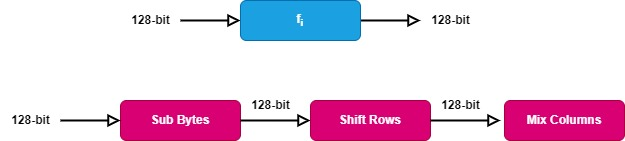
\includegraphics[width = 17cm]{Round Function of AES.jpg}
	\end{center}
	\subsection{Sub bytes}
	\centering Sub bytes : \{0, 1\}$^{128} \rightarrow$ \{0, 1\}$^{128}$\\\flushleft
	S $\rightarrow$ input.\vspace{0.2cm}\\
	\centering S $\rightarrow$ 
	\begin{tabular}{| c c c c |}
		S\textsubscript{00} & S\textsubscript{01} & S\textsubscript{02} & S\textsubscript{03}\\
		S\textsubscript{10} & S\textsubscript{11} & S\textsubscript{12} & S\textsubscript{13}\\
		S\textsubscript{20} & S\textsubscript{21} & S\textsubscript{22} & S\textsubscript{23}\\
		S\textsubscript{30} & S\textsubscript{31} & S\textsubscript{32} & S\textsubscript{33}
	\end{tabular}\vspace{0.2cm}\\
	S\textsubscript{ij} $\rightarrow$ 8 bit.\\
	\flushleft
	P $\rightarrow$ Plain text 128 bit.\vspace{0.2cm}\\
	P $\rightarrow$ 
	\begin{tabular}{| c c c c |}
		P\textsubscript{0} & P\textsubscript{4} & P\textsubscript{8} & P\textsubscript{12}\\
		P\textsubscript{1} & P\textsubscript{5} & P\textsubscript{9} & P\textsubscript{13}\\
		P\textsubscript{2} & P\textsubscript{6} & P\textsubscript{10} & P\textsubscript{14}\\
		P\textsubscript{3} & P\textsubscript{7} & P\textsubscript{11} & P\textsubscript{15}
	\end{tabular} 
	+ K\textsubscript{1} $\rightarrow$ (S\textsubscript{ij})\textsubscript{$4x4$} \hfill len(P\textsubscript{i}) = 8 bit\vspace{0.2cm}\\
	K\textsubscript{1} $\rightarrow$ 128 bit. K\textsubscript{0}, K\textsubscript{1},..., K\textsubscript{15}\vspace{0.2cm}\\ 
	K\textsubscript{1} $\rightarrow$ 
	\begin{tabular}{| c c c c |}
		K\textsubscript{0} & K\textsubscript{4} & K\textsubscript{8} & K\textsubscript{12}\\
		K\textsubscript{1} & K\textsubscript{5} & K\textsubscript{9} & K\textsubscript{13}\\
		K\textsubscript{2} & K\textsubscript{6} & K\textsubscript{10} & K\textsubscript{14}\\
		K\textsubscript{3} & K\textsubscript{7} & K\textsubscript{11} & K\textsubscript{15}
	\end{tabular} 
	\subsection{Sub bytes}
	S = (S\textsubscript{ij})\textsubscript{$4x4$}\\
	S : \{0, 1\}$^{8} \rightarrow$ \{0, 1\}$^{8}$ \hspace{1cm} S(0) = 0\\
	\begin{enumerate}[label=\roman*.]
		\item (c\textsubscript{7}c\textsubscript{6}c\textsubscript{5}c\textsubscript{4}c\textsubscript{3}c\textsubscript{2}c\textsubscript{1}c\textsubscript{0}) = (01100011) = (63)\textsubscript{16}
		\item S(S\textsubscript{ij}) = (a\textsubscript{7}a\textsubscript{6}a\textsubscript{5}a\textsubscript{4}a\textsubscript{3}a\textsubscript{2}a\textsubscript{1}a\textsubscript{0})
		\item For i = 0 to 7 \\ \hspace{0.6cm} b\textsubscript{i} = (a\textsubscript{i} + a\textsubscript{(i+4)\%8} + a\textsubscript{(i+5)\%8} + a\textsubscript{(i+6)\%8} + a\textsubscript{(i+7)\%8} + c\textsubscript{i}) mod 2
		\item (b\textsubscript{7}b\textsubscript{6}b\textsubscript{5}b\textsubscript{4}b\textsubscript{3}b\textsubscript{2}b\textsubscript{1}b\textsubscript{0})
		\item S$^1$\textsubscript{ij} = (b\textsubscript{7}b\textsubscript{6}b\textsubscript{5}b\textsubscript{4}b\textsubscript{3}b\textsubscript{2}b\textsubscript{1}b\textsubscript{0})
	\end{enumerate}
	$\bullet$ S : \{0, 1\}$^{8} \rightarrow$ \{0, 1\}$^{8}$ \hspace{1cm} S(0) = 0\\
	X $\neq$ 0 $\in$ \{0, 1\}$^{8}$\\
	S(X) = Y $\in$ \{0, 1\}$^{8}$\\
	X = (a\textsubscript{7}a\textsubscript{6}a\textsubscript{5}a\textsubscript{4}a\textsubscript{3}a\textsubscript{2}a\textsubscript{1}a\textsubscript{0}), a\textsubscript{i} $\in$ \{0, 1\}\\
	P(x) = a\textsubscript{0} + a\textsubscript{1}$x$ + a\textsubscript{2}$x^2$ + ... + a\textsubscript{7}$x^7$\\
	deg(P(x)) $\leq$ 7\\
	P(x) $\in$ F\textsubscript{2}[$x$]\hfill
	g(x) = $x^8$ + $x^4$ + $x^3$ + $x$ + 1\\\hfill g(x) is a primitive polynomial.\\
	(F\textsubscript{2}[x]/$<g(x)>$, +, $\ast$) $\rightarrow$ Field.\\
	Find the multiplicative inverse of P(x) under modulo ($x^8$ + $x^4$ + $x^3$ + $x$ + 1)\vspace{0.2cm}\\
	p(x).q(x) = 1 mod ($x^8$ + $x^4$ + $x^3$ + $x$ + 1)\\
	$\Rightarrow$ p(x).q(x) - 1 = h(x).($x^8$ + $x^4$ + $x^3$ + $x$ + 1)\\
	1 = p(x).q(x) + h\textsubscript{1}(x).($x^8$ + $x^4$ + $x^3$ + $x$ + 1)\vspace{0.2cm}\\
	gcd(a, b) = as + bt\\
	gcd(P(x), $x^8$ + $x^4$ + $x^3$ + $x$ + 1) = 1\vspace{0.2cm}\\
	How to find g(x) ?\\
	$\Rightarrow$ Extended Euclidean Algorithm finds q(x)\\
	q(x) $\rightarrow$ deg(q(x)) $\leq$ 7\\
	q(x) = r\textsubscript{0} + r\textsubscript{1}$x$ + r\textsubscript{2}$x^2$ + ... + r\textsubscript{7}$x^7$\\
	q(x) $\rightarrow$ (r\textsubscript{7}r\textsubscript{6}r\textsubscript{5}r\textsubscript{4}r\textsubscript{3}r\textsubscript{2}r\textsubscript{1}r\textsubscript{0}) $\in$ \{0, 1\}$^{8}$\\
	S(x) = Y = (r\textsubscript{7}r\textsubscript{6}r\textsubscript{5}r\textsubscript{4}r\textsubscript{3}r\textsubscript{2}r\textsubscript{1}r\textsubscript{0})\\
	\subsection*{Example}
	Find S(01010011) = ?\\
	p(x) = $x^6$ + $x^4$ + $x$ + 1\\
	g(x) = $x^8$ + $x^4$ + $x^3$ + $x$ + 1\vspace{0.2cm}\\
	$x^6$ + $x^4$ + $x$ + 1) $x^8$ + $x^4$ + $x^3$ + $x$ + 1 ($x^2$ + 1\\
	\hspace*{3cm} $x^2 + x + 1$\\
	\hspace*{3cm} \xdash[9.8em]\\
	\hspace*{3cm} $x^6$ + $x^4$ + $x^2$ + $x$ + 1\\
	\hspace*{3cm} $x^6$ + $x^4$ + $x$ + 1\\
	\hspace*{3cm} \xdash[9.8em]\\
	\hspace*{4.6cm} $x^2$) $x^6$ + $x^4$ + $x$ + 1 ( $x^4$ + $x^2$\\
	\hspace*{5.26cm} $x^6$ \\
	\hspace*{5.26cm} \xdash[6em]\\
	\hspace*{5.26cm} $x^4$ + $x$ + 1\\
	\hspace*{5.26cm} $x^4$\\
	\hspace*{5.26cm} \xdash[6em]\\
	\hspace*{6cm} $x$ + 1) $x^2$ ($x$ + 1\\
	\hspace*{7cm} $x^2$ + $x$\\
	\hspace*{7cm} \xdash[3.5em]\\
	\hspace*{7.5cm} $x$\\
	\hspace*{7.5cm} $x + 1$\\
	\hspace*{7.2cm} \xdash[3.5em]\\
	\hspace*{8cm} 1\\
	\hspace*{7.2cm} \xdash[3.5em]\\
	1 = $x^2$ + ($x + 1$)($x + 1$)\\
	\hspace{0.3cm}= $x^2$ + ($x + 1$)[($x^6$ + $x^4$ + $x$ + 1) + $x^2$($x^4$ + $x^2$)]\\
	\hspace{0.3cm}= $x^2$[$x^5 + x^4 + x^3 + x^2 +$ 1] + ($x + 1$)[($x^6$ + $x^4$ + $x$ + 1)]\\
	\hspace{0.3cm}= [($x^8$ + $x^4$ + $x^3$ + $x$ + 1) + ($x^6$ + $x^4$ + $x^2$ + $x$ + 1)($x^2$ + 1)][$x^5 + x^4 + x^3 + x^2 +$ 1] + \hspace*{0.8cm}($x + 1$)[($x^6$ + $x^4$ + $x$ + 1)] \\
	1 = [($x^6$ + $x^4$ + $x$ + 1)][($x^2$ + 1)($x^5 + x^4 + x^3 + x^2 +$ 1) + ($x$ + 1)] + [($x^8$ + $x^4$ + $x^3$ + $x$ + \hspace*{0.8cm}1)][($x^5 + x^4 + x^3 + x^2 +$ 1)]\vspace{0.2cm}\\
	Co-efficient of ($x^6$ + $x^4$ + $x$ + 1) is multiplicative inverse of p(x) (i.e., q(x))\\
	So, q(x) = ($x^2$ + 1)($x^5 + x^4 + x^3 + x^2 +$ 1) + ($x$ + 1)\\
	\hspace{1.5cm}= ($x^7$ + $x^6$ + $x^5$ + $x^4$ + $x^2$ + $x^5 + x^4 + x^3 + x^2 +$ 1) + ($x$ + 1)\\
	\hspace{1.5cm}= $x^7$ + $x^6$ + $x^3$ + $x$\\
	(11001010) $\rightarrow$ output.\\
	c = (01100011)\\
	b\textsubscript{i} = (a\textsubscript{i} + a\textsubscript{(i+4)\%8} + a\textsubscript{(i+5)\%8} + a\textsubscript{(i+6)\%8} + a\textsubscript{(i+7)\%8} + c\textsubscript{i}) mod 2\\
	b\textsubscript{0} = (a\textsubscript{0} + a\textsubscript{4} + a\textsubscript{5} + a\textsubscript{6} + a\textsubscript{7} + c\textsubscript{0}) mod 2\\
	\hspace{0.55cm}= (0 + 0 + 0 + 1 + 1 + 1)mod2\\
	\hspace{0.55cm}= 1\\
	b\textsubscript{1} = (a\textsubscript{1} + a\textsubscript{5} + a\textsubscript{6} + a\textsubscript{7} + a\textsubscript{0} + c\textsubscript{1}) mod 2\\
	\hspace{0.55cm}= (1 + 0 + 1 + 1 + 0 + 1)mod2\\
	\hspace{0.55cm}= 0\\
	b\textsubscript{2} = 1\\
	b\textsubscript{3} = 1\\
	b\textsubscript{4} = 0\\
	b\textsubscript{5} = 1\\
	b\textsubscript{6} = 1\\
	b\textsubscript{7} = 1\\
	Output of Sub bytes (1110 1101)\\
	\hspace{4cm} E\hspace{0.5cm}D\\
	Subbytes ( 0101 0011 ) = ( 1110 1101 )\\
	Subbytes ( 53 ) = ( ED )\vspace{0.2cm}\\
	\subsection{AES S-Boxes}
	\begin{tabular}{| c | c | c | c | c | c | c | c | c | c | c | c | c | c | c | c | c |}
		\hline 
		&0 & 1 &2& 3 &4 &5& 6& 7& 8 &9&A&B&C&D&E&F\\
		\hline 
		0 &63 &7C &77 &7B& F2& 6B& 6F& C5 &30 &01 &67 &2B &FE &D7 &AB &76\\
		\hline
		1& CA& 82& C9& 7D &FA &59 &47& F0 &AD &D4 &A2 &AF &9C &A4 &72 &C0\\
		\hline
		2 &B7 &FD &93 &26 &36 &3F &F7 &CC &34 &A5 &E5 &F1 &71 &D8 &31 &15\\
		\hline
		3& 04 &C7 &23 &C3 &18 &96 &05 &9A &07 &12 &80 &E2 &EB &27 &B2& 75\\
		\hline
		4& 09& 83& 2C& 1A& 1B& 6E& 5A& A0& 52& 3B& D6& B3& 29& E3& 2F& 84\\
		\hline
		5 &53 &D1 &00 &ED& 20& FC& B1& 5B &6A& CB &BE &39& 4A& 4C &58& CF\\
		\hline
		6& D0 &EF &AA &FB &43 &4D &33 &85 &45 &F9 &02 &7F &50 &3C &9F &A8\\
		\hline
		7 &51 &A3 &40 &8F &92 &9D &38 &F5 &BC &B6 &DA &21 &10& FF& F3& D2\\
		\hline
		8 &CD &0C &13 &EC &5F &97 &44 &17 &C4 &A7 &7E &3D &64 &5D &19 &73\\
		\hline
		9 &60 &81 &4F &DC &22 &2A &90 &88 &46 &EE &B8 &14 &DE &5E &0B &DB\\
		\hline
		A &E0 &32 &3A &0A &49 &06 &24 &5C &C2 &D3 &AC &62 &91 &95 &E4 &79\\
		\hline
		B &E7 &C8 &37 &6D &8D &D5 &4E &A9 &6C &56 &F4 &EA &65 &7A &AE &08\\
		\hline
		C &BA &78 &25 &2E &1C &A6 &B4 &C6 &E8 &DD &74 &1F &4B &BD &8B &8A\\
		\hline
		D &70 &3E &B5 &66 &48 &03 &F6 &0E &61 &35 &57 &B9 &86 &C1 &1D &9E\\
		\hline
		E &E1 &F8 &98 &11 &69 &D9 &8E &94 &9B &1E &87 &E9 &CE &55 &28 &DF\\
		\hline
		F &8C &A1 &89 &0D &BF &E6 &42 &68 &41 &99 &2D &0F &B0 &54 &BB &16\\
		\hline
	\end{tabular}\vspace{0.1cm}
	\centering\textbf{(a) S-box}\flushleft
	
	\begin{tabular}{| c | c | c | c | c | c | c | c | c | c | c | c | c | c | c | c | c |}
		\hline 
		&0 &1  &2 &3 &4 &5 &6 &7 &8 &9 &A &B &C &D &E &F\\
		\hline
		0 &52 &09 &6A &D5 &30 &36 &A5 &38 &BF &40 &A3 &9E &81 &F3 &D7 &FB\\
		\hline
		1 &7C &E3 &39 &82 &9B &2F &FF &87 &34 &8E &43 &44 &C4 &DE &E9 &CB\\
		\hline
		2 &54 &7B &94 &32 &A6 &C2 &23 &3D &EE &4C &95 &0B &42 &FA &C3 &4E\\
		\hline
		3 &08 &2E &A1 &66 &28 &D9 &24 &B2 &76 &5B &A2 &49 &6D &8B &D1 &25\\
		\hline
		4 &72 &F8 &F6 &64 &86 &68 &98 &16 &D4 &A4 &5C &CC &5D &65 &B6 &92\\
		\hline
		5 &6C &70 &48 &50 &FD &ED &B9 &DA &5E &15 &46 &57 &A7 &8D &9D &84\\
		\hline
		6 &90 &D8 &AB &00 &8C &BC &D3 &0A &F7 &E4 &58 &05& B8& B3 &45 &06\\
		\hline
		7 &D0 &2C &1E &8F &CA &3F &0F &02 &C1 &AF &BD &03 &01 &13 &8A &6B\\
		\hline
		8 &3A &91 &11 &41 &4F &67 &DC &EA &97 &F2 &CF &CE &F0 &B4 &E6 &73\\
		\hline
		9 &96 &AC &74 &22 &E7 &AD &35 &85 &E2 &F9 &37 &E8 &1C &75 &DF &6E\\
		\hline
		A &47 &F1 &1A &71 &1D &29 &C5 &89 &6F &B7 &62 &0E &AA &18 &BE &1B\\
		\hline
		B &FC &56 &3E &4B &C6 &D2 &79 &20 &9A &DB &C0 &FE &78 &CD &5A &F4\\
		\hline
		C &1F &DD &A8 &33 &88 &07 &C7 &31 &B1 &12 &10 &59 &27 &80 &EC &5F\\
		\hline
		D &60 &51 &7F &A9 &19 &B5 &4A &0D &2D &E5 &7A &9F &93 &C9 &9C &EF\\
		\hline
		E &A0 &E0 &3B &4D &AE &2A &F5 &B0 &C8& EB &BB &3C &83 &53 &99 &61\\
		\hline
		F &17 &2B &04& 7E &BA &77 &D6 &26 &E1 &69 &14 &63 &55 &21 &0C &7D\\
		\hline
	\end{tabular}\vspace{0.1cm}
	\centering\textbf{(b) Inverse S-box}\flushleft
\end{document}